\documentclass[12pt,onecolumn,a4paper]{report}
\usepackage{epsfig,graphicx,subfigure,amsthm,amsmath}
\usepackage{color,xcolor}     
\usepackage{xepersian}
\usepackage{graphicx}
\usepackage{sectsty}
\usepackage{hyperref}
\settextfont[]{B-NAZANIN.TTF}
\setlatintextfont[Scale=1]{Times New Roman}
\usepackage{geometry}
 \geometry{
 a4paper,
 total={170mm,257mm},
 left=20mm,
 top=20mm,
 }

\begin{document}
%\text{گزارش پروژه کارشناسی}
\title{
\includegraphics[width=5cm, height= 5cm]{3.jpg}\\\Large{دانشکده فیزیک}\\{\LARGE{گزارش پروژه کارشناسی}}\\{\\{\Huge{عنوان پروژه:}\\\Huge{شبیه سازی برهمکنش غشا لیپیدی و نانو ذرات \\با استفاده از نرم افزار \lr{VCM} }}} }
\author{\LARGE{استاد پروژه : دکتر محمدرضا اجتهادی}\\\LARGE{یگانه بهاری - فهیمه فخری}}
\date{\LARGE{\today}}
\maketitle
\tableofcontents

\section{\LARGE{مقدمه} }
\large{غشای سلولی شامل دو لایه فسفولیپیدی همراه با پروتئین است. مولکول فسفولیپید از اتصال یک سر شامل گروه فسفات
به یک یا دو زنجیره هیدروکربنی تشکیل شده است
مولکول های چربی با قرار دادن زنجیره هیدروکربنیشان
رودرروی یکدیگر، تشکیل یک غشای دو لایه میدهند.سر شامل گروه فسفات دارای خاصیت آبدوستی و دم شامل زنجیره هیدروکربنی دارای خاصیت
آبگریزی است. با تجمع پروتئینهای شامل ساختار
آب گریز بر یک طرف غشا، دم آبگریز این پروتئینها وارد غشای لیپیدی (یعنی ناحیه
شامل زنجیره های هیدروکربنی) میشود ومیتواند منجر به ایجاد
انحنا در غشا شود.ورود و خروج بسیاری از باکتری ها به صورت نانوذره به این صورت رخ میدهد.\\
تمرکز این پروژه روی شبیه سازی برهمکنش غشا با آن دسته از نانوذراتی است که بدون استفاده از عوامل خارجی و فقط به کمک جاذبه میان غشا و ذرات باعث تغییر شکل غشا میشوند.
هدف اصلی مشاهده دینامیک سیستم برهمکنش غشا و نانوذرات است که به کمک نرم افزار\lr{VCM}  انجام میشود.
ما در طول انجام این پروژه تجربیاتی کسب کرده ایم و کارهایی انجام داده ایم که در طول این گزارش به آنها اشاره خواهیم کرد. در نهایت با مقادیری که برای پارامتر های مربوطه پیدا کرده و به دست آورده بودیم موفق به مشاهده حرکت نانوذرات بر روی غشا و نزدیک شدن دو نانوذره به یکدیگر شدیم.
در آخر تشکر بسیار از دکتر اجتهادی و آقای علی فرنودی داریم که صبورانه در این پروژه ما را همراهی و راهنمایی کردند و آموخته های بسیاری را به ما ارزانی داشتند.}



\section{\LARGE{نصب و شروع کار با نرم افزار}}
\large{در ابتدا این را بدانید که بهتر است نرم افزار را روی سیستم عامل لینوکس نصب کنید. ما از بین توزیع های لینوکس اوبونتو را انتخاب کردیم. اگر سیستم عامل ویندوز دارید میتوانید به راحتی منابع فارسی و انگلیسی در اینترنت برای راهنمایی نصب اوبونتو بر روی سیستم عامل ویندوز پیدا کنید. اما در مراحل نصب نرم \lr{VCM} نتوانستیم \lr{Opencl} را بر روی اوبونتو 20 نصب کنیم. در حالی که نصب \lr{Opencl} بر روی اوبونتو 18 و 16 ممکن بود. و یکی از ما با اوبونتو 18 و دیگری با اوبونتو 16 شروع به کار کردیم. نسخه \lr{Opencl} ای که نصب کردیم را روی گیت هاب به اشتراک گذاشته ایم. به هنگام به کار گرفتن برهمکنش در استفاده از نرم افزار \lr{VCM} در اوبونتو 18 این نسخه \lr{Opencl} کار نمیکند. \\
برای مراحل بعدی نرم افزار میتوانید از راهنمای نصب سایت نرم افزار استفاده کنید.
}




\section{\LARGE{طرح مساله}}
در مساله شبیه سازی غشا سلولی به به وسیله نرم افزار ابتدا باید تمام واحد های مورد نظر را به واحد های مورد قبول نرم افزار تبدیل کنیم. از نظر فیزیکی مدلسازی غشا به این صورت انجام میشود که غشا از یک سری فنر های متصل  بهم تشکیل شده است که دارای سختی فنر و سختی خمشی هستند که کل سیستم در یک حمام گرمای قرار دارد .برای شبیه سازی باید معدله نیروی وارد به این فنر ها را حل کنیم تا بتوانیم دینامیک سیستم را پیش بینی کنیم.\\

\lr{VCM} یک بسته نرمافزاری برای انجام شبیهسازی های دینامیک مولکولی است که قادر است
با مدلسازی درشتدانه اجزای مختلف سلول، خواص مکانیکی اجزای سلول را بررسی کند.
% \lr{VCM}ای در دستگاه واحدهای کاهیده صورت میگیرد، 
از آنجا که مدلسازی در \lr{VCM}در دستگاه واحد های کاهیده صورت میگیرد در هر مساله با ترجمه واحد های مورد نظر به واحد های قابل قبول نرم افزار میتوان طیف وسیعی از فرایند های بیولوژیکی را شبیه سازی کرد.\\
در این پروژه تلاش کردیم تا با جستجو و یافتن پارامتر های واقعی غشا و نانوذرات همانند سختی خمش و سختی فنر  تبدیل آن ها به واحد های نرم افزار یک شبیه سازی واقعی انجام دهیم.




\section{\LARGE{روش شبیه سازی}}
به عنوان یک پیشنیاز برای اشنایی بیشتر با نرم افزار ابتدا از یک مش بندی آماده استفاده کرده و به  وسیله الگوریتم های گفته شده دینامیک سیستم فنر های در حل نوسان را شبیه سازی کردیم و نوسان فنر ها را مشاهده کردیم که با معادلات نیوتن سازگار است.نمودار میانگین شعاع این غشا در طول زمان به صورت زیر است\\.
\begin{center}
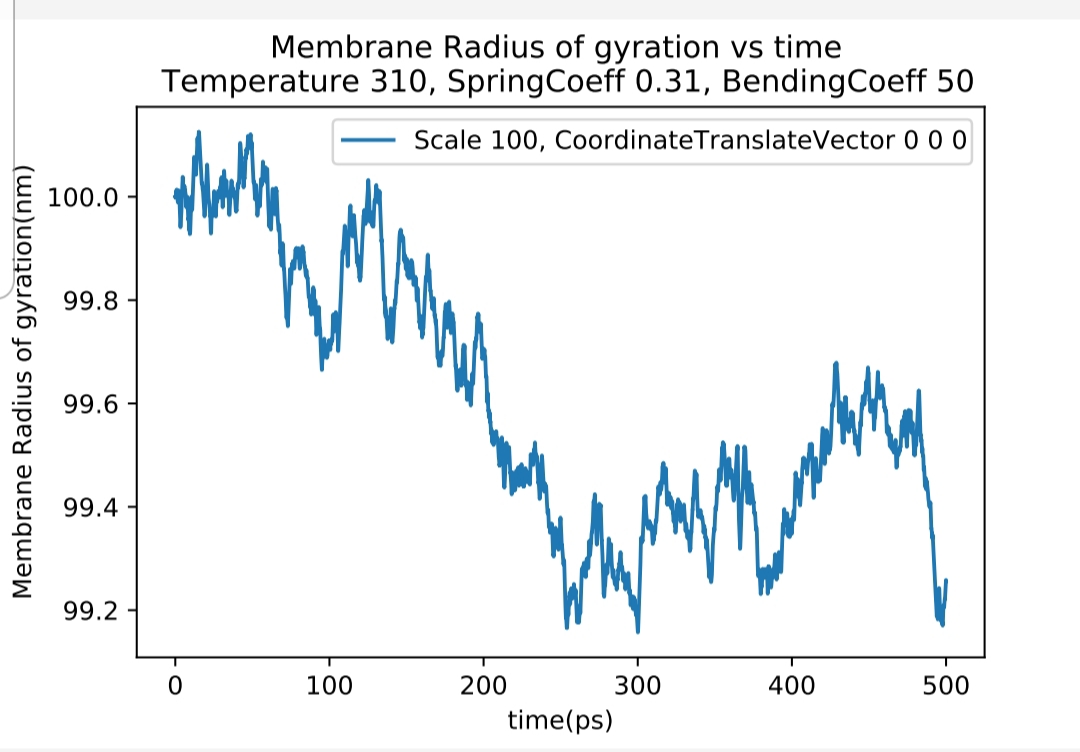
\includegraphics[width=11cm, height=9cm]{20210215_142631.jpg}
\end{center}\\

\begin{center}
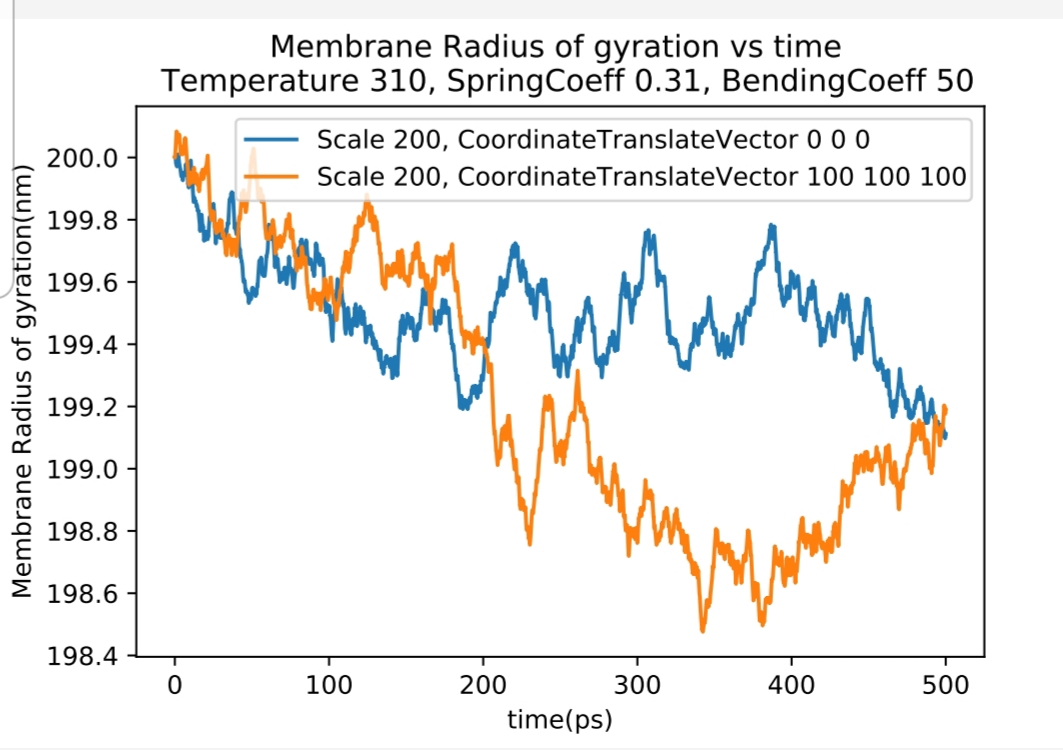
\includegraphics[width=11cm, height=9cm]{20210215_142645.jpg}
\end{center}\\
پس از این مقدمات
برای حل این مساله ابتدا تلاش کردیم تا به وسیله جستجو و مطالعه واحد های واقعی مورد نظر را بیابیم. برای بدست آوردن پارامتر های غشا نرم افزار\lr{VCM}غشای لیپیدی را به وسیله مش بندی مثلثی شبیه سازی میکند به این صورت که بین هر دو نقطه از شبکه یک فنر هارمونیک وجود داردو بین هر دو فنر همسایه نیز پتانسیل خمشی اعمال میشود.مجموع این دو پتانسیل خواص کشسان غشا را به وجود می آورد.
در شبیه سازی به وسیله روش دینامیک مولکولی باید معدلات حاکم بر ذرات تشکیل دهنده سیستم را حل کنیم .یکی از الگوریتم های معمول د راین نوع شبیه سازی الگوریتم ورله سرعتی است که در سیستم های زیستی  در صورت استفاده از این الگوریتم باید برای سیستم ترموسات تعریف شود تا دما ثابت بماند . اما ترموستات اگرچه دما را ثابت میکند اما نمیتواند  حرکات ذرات بر اثر افت و خیز را شبیه سازی کند . یک راه حل مناسب استفاده از دینامیک لانژون است به این ترتیب که با حل این معادله میتوان سیستم غوطه ور در حمام گرمایی را شبیه سازی کرد.\\
در ابتدا باید محیط متناسب برای غشا را با توجه به انچه در آزمایشگاه مشاهده کردیم اعم از دمای محیط و روش حل معادلات حاکم بر سیستم را  در نرم افزار مشخص کنیم.پس از آن به سراغ تنظیم پارامتر های غشا میرویم.\\
غشاهای زیستی به دلیل پخش سطحی مولکولهای
چربی سازنده شان، مانند مایع دوبعدی عمل میکنند. این خاصیت با تغییر اتصال نقاط شبکه
در طی شبیهسازی بازنمایی میشود.طی این فرآیند، انرژی مکانیکی غشا از طریق انتخاب های
مونت-کارلو برای یافتن بهترین پیکربندی شبکه کمینه میشود.
در نتیجه برای شبیه سازی غشا لیپیدی که فیزیک آن شبیه غشای لیپیدی واقعی دیده شده در آزمایشگاه باشد باید پارامتر های سایز غشا  و سختی خمشی و سختی فنر را بدست آوریم .برای بدست آوردن واحد ها به مقالات مختلفی که در انتهای گزارش به آن ها ارجاع داده شده رجوع کردیم و با استفاده از شهود خود به عنوان فیزیک پیشه واحد ها را بدست آوردیم.\\
برای شبیه سازی نانوذارت باید ابعاد آن ها را در نظر بگیریم و با توجه به سایز غشا آن ها را تنظیم کنیم.این ذرات انعطاف پذیری بسیار کمتری از غشا دارند و نوعی جسم صلب به حساب می آیند و تنها میتوانند حرکت انتقالی و دورانی حول مرکز جرم خود انجام دهند .در این پروژه این نانوذارت را مشابه با غشا شبیه سازی کرده اما سختی فنر و سختی خمشی آن ها زا به گونه ای تنظیم کرده که به صورت جسم صلب باشند.برای جلوگیری از فرو رفتن نانوذرات در یک دیگر بینشان یک پتانسیل تعریف کرده ایم. \\
یکی از چالش های مهم این پروژه تنظیم برهمکنش میان غشا و نانوذرات و بررسی دینامیک سیستم است. برای این برهمکنش از پتانسیل لنارد جونز استفاده کرده ایم. این پتانسیل برای برهمکنش های کوتاه برد میان غشا و نانو ذرات مناسب است.




\section{\LARGE{تبدیل واحد}}
مقادیری  که از مقاله بدست آوردیم برای ویژگی های مکانیکی غشا بزرگ به صورت زیر است :
\begin{center}
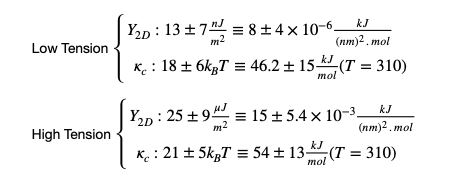
\includegraphics[width=13cm, height=6cm]{IMG_20210215_210004_891.jpg}
\end{center}\\
برای تبدیل مدول یانگ دو بعدی به سختی فنر و تبدیل سختی خمشی اندازه گیری شده به سختی خمشی مطلوب نرم افزار از رابطه  زیر که در شبکه های مثلثی برقرار است استفاده میکنیم:
\begin{center}
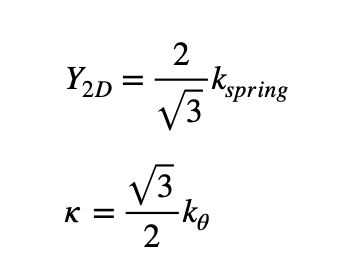
\includegraphics[width=6cm, height=4cm]{IMG_20210215_210007_241 (1).jpg}
\end{center}\\
شعاع غشا بزرگ برابر 8000 نانومتر است برای افزایش سرعت شبیه سازی و نتیجه گیری هر 400 نانومتر را برابر یک در نظر میگیریم و متناسب با آن مقادیر سختی فنر و سختی خمشی را نیز تنظیم میکنیم و شبیه سازی را به وسیله این پارامتر ها آغاز میکنیم




\section{\LARGE{نتایج شبیه سازی}}
برای آماده سازی چیدمان سیستم غشا و فضای اطراف دما را 310 کلوین در نظر گرفتیم و از یک مش بندی با 2562 راس استفاده کردیم. شعاع نانوذارت نیز 1/20 برابر شعاع غشا است.\\
در قدم اول پس از بدست آوردن پارامتر ها فقط غشا را شبیه سازی کردیم.
 و به علت وجود مش
 بندی مثلثی و خاصیت پخش رئوس دو نوع ساختار غشا در شبیه سازی دیده میشود که بر اثر حضور یا عدم حضور این خاصیت به وجود آمده اند. که به  ترتیب به آن ها غشای کشسان و مایع میگوییم.
 در شکل زیر نمونه ای از هر دو غشا را مشاهده میکنیم.
 
%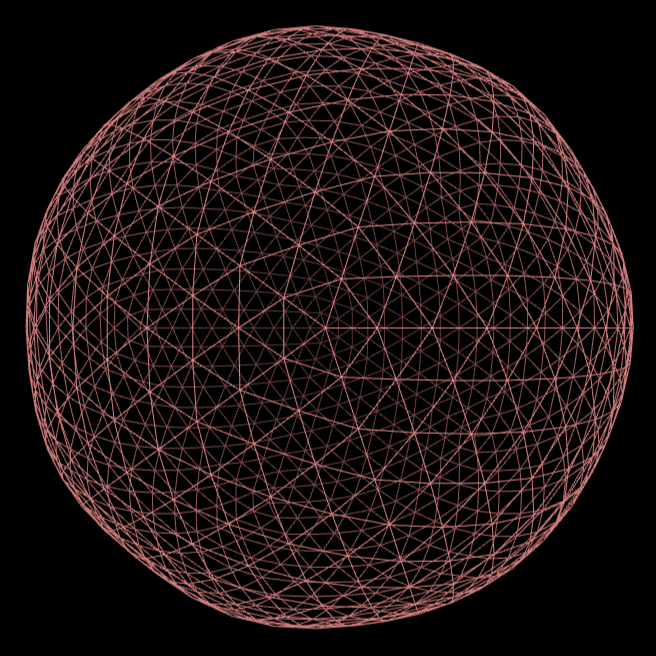
\includegraphics{1.png}
\begin{center}
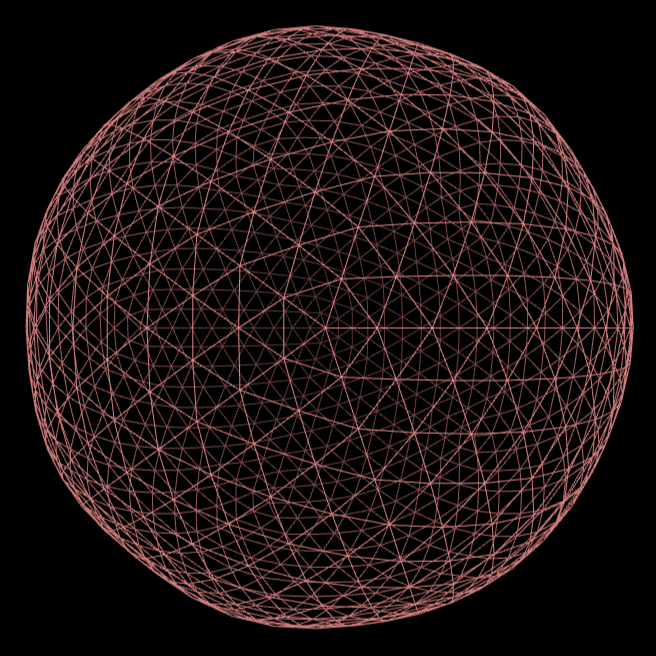
\includegraphics[width=9cm, height=9cm]{1.png}
\end{center}\\

\begin{center}
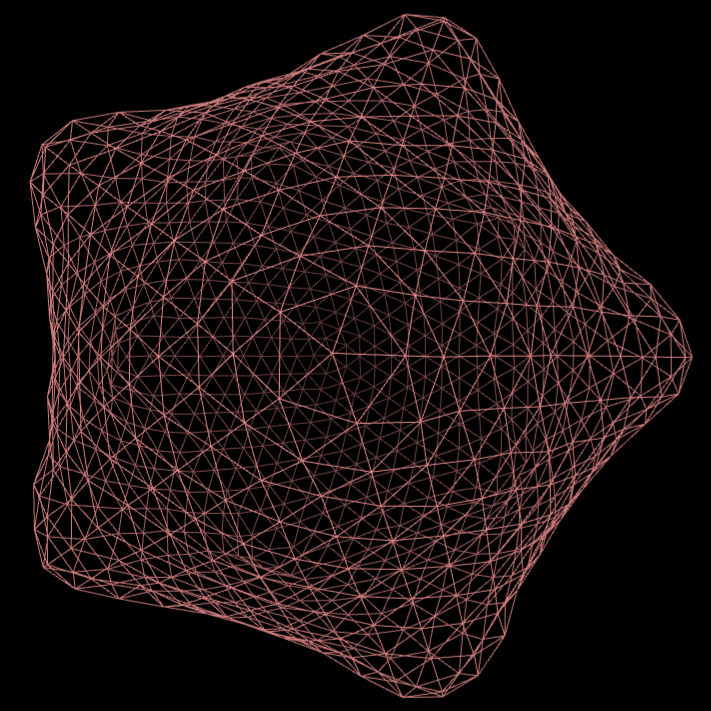
\includegraphics[width=9cm, height=9cm]{2.png}
\end{center}\\

\\
در قدم بعدی به شبیه غشا نانوذرات را نیز اضافه کردیم. در این مرحله علاوه بر تنظیم پارامتر های فبل باید واحد های مورد نیاز برهمکنش لنارد جونز را هم تنظیم کنیم.

در شکل زیر سایز نانوذره را در مقایسه با سایز غشا مشاهده میکنیم
در این شکل برهمکنشی بین غشا و نانوذره تعریف نشده و صرفا برای مقایسه ابعاد و یکسان بود ساختار غشا و نانوذرات نشان داده شده است.
\\.
\begin{center}
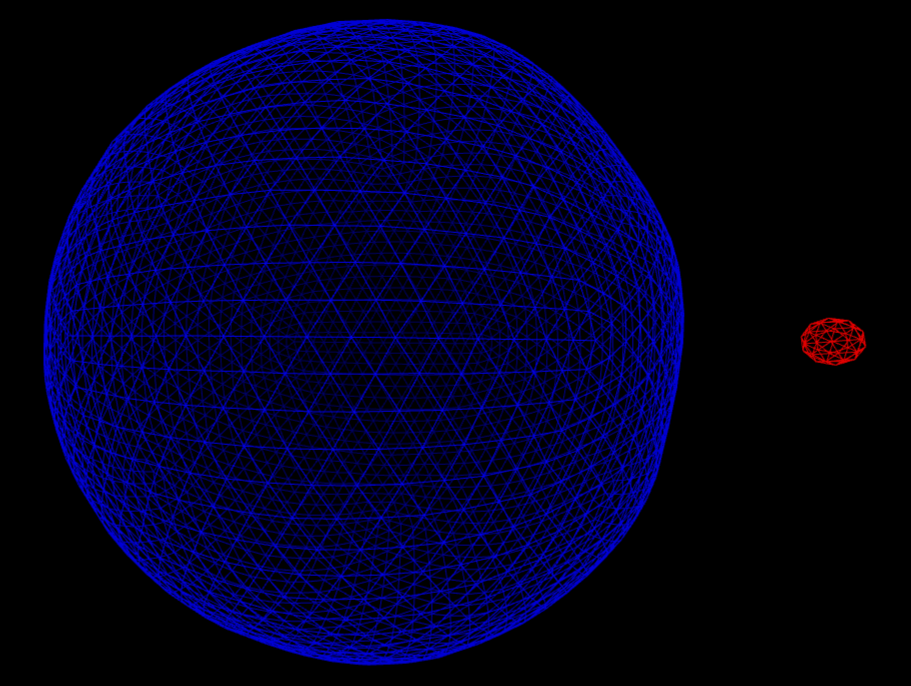
\includegraphics[width=11cm, height=9cm]{20210209_195305.png}
\end{center}\\

در ادامه برهمکنش غشا نانوذرات را   بررسی میکنیم
ابتدا یک نانو ذره را همراه غشا شبیه سازی میکنیم.
در این برهمکنش با توجه به اینکه از پتانسیل لنارد جونز استفاده شده و پارامتر های مهم این پتانسیل نیز عمق چاه و سیگما است \\
%نظیمن پارامتر ها  میتوان برهمکنش را مشاهده کرد%%% 
با تنظیم پارامتر های برهمکنش غشا با یک نانو ذره با توجه به عمق چاه پتانسیل لنارد جونز نانو ذره ابتدا درون غشا رها میشود و پس از آن به دیواره غشا میچسبد.
با توچه به شکل های نشان داده شده نانوذره ابتدا درون غشا و سپس به دیواره چسبیده است.
\begin{center}
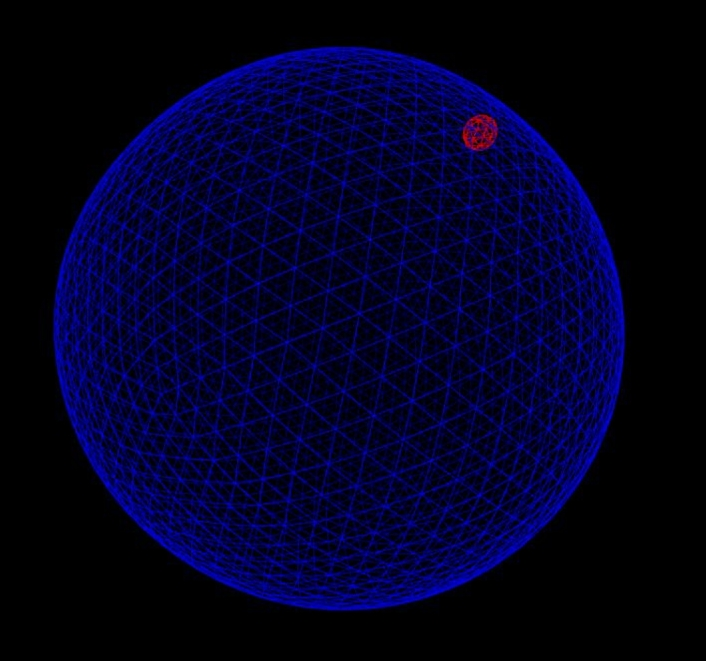
\includegraphics[width=9cm, height=9cm]{20210214_160511.jpg}
\end{center}\\
\begin{center}
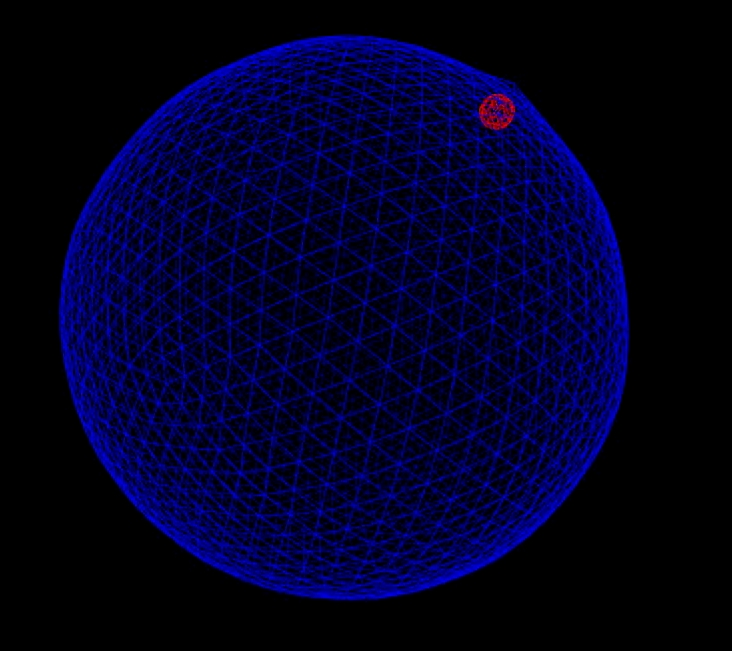
\includegraphics[width=9cm, height=9cm]{20210214_160439.jpg}
\end{center}\\

پس از مشاهده برهمکنش غشا و یک نانو ذره به سراغ مشاهده ی سیستم با دو نانو ذره میرویم.با افزایش قدرت پتانسیل برهمکنش مشاهده میکنیم که غشا به 
دور نانوذرات پیچیده شده است.
\begin{center}
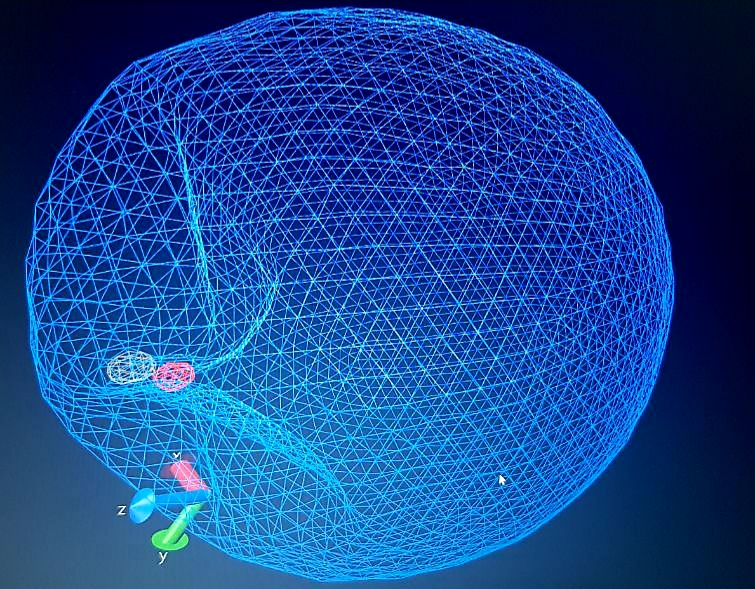
\includegraphics[width=11cm, height=9cm]{20210213_204324.jpg}
\end{center}\\




\begin{center}
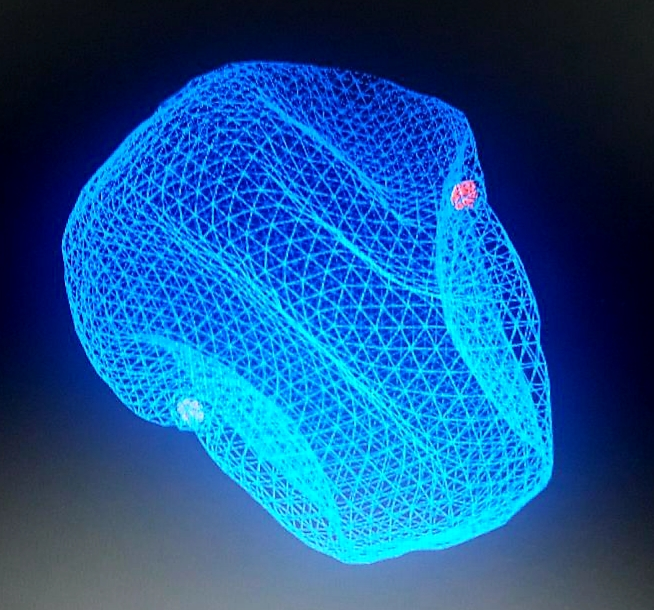
\includegraphics[width=11cm, height=9cm]{20210213_204232.jpg}
\end{center}\\


با توجه به نتایج شبیه سازی بسیار محتمل است که در برهمکنش غشا با دو نانوذره نانوذرات به یک دیگر نزدیک شوند . با توجه به اینکه هیچ نسرو جاذبه ای بین نانوذرات تعریف نشده ااین نزدیک شدن به علت به وجود آمدن نیروی موثری است که از برهمکنش همزمان غشا با نانوذره ایجاد میشود .در نتیجه غشا هزینه انرژی خمشی کمتری برای در بر گرفتن نانوذرات هزینه میکند.\\
در شکل های زیر مشاهده میکنیم که دو نانوذره به یک دیگر نزدیک شده اند.
شکل اول مکان اولیه نانوذرات را نشان میدهد.
شکل بعدی پس از 337 پیکو ثانیه شبیه سازی شده است.
\begin{center}
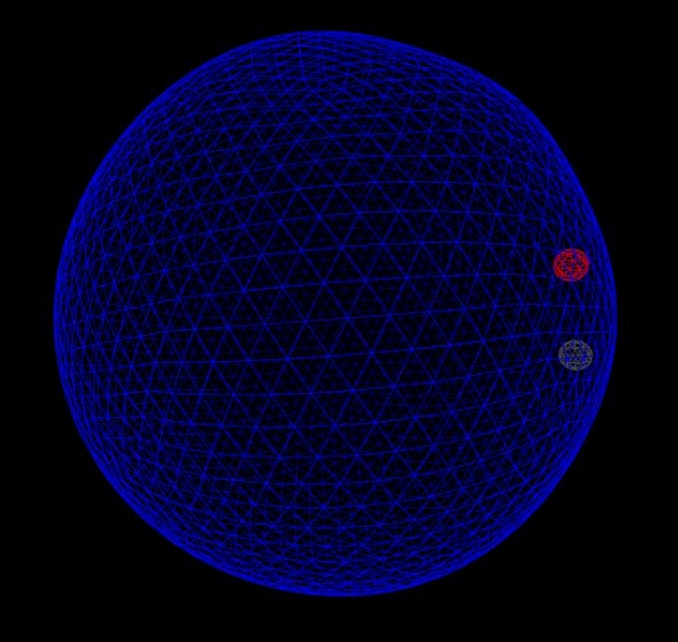
\includegraphics[width=9cm, height=9cm]{20210215_152251.jpg}
\end{center}\\

\begin{center}
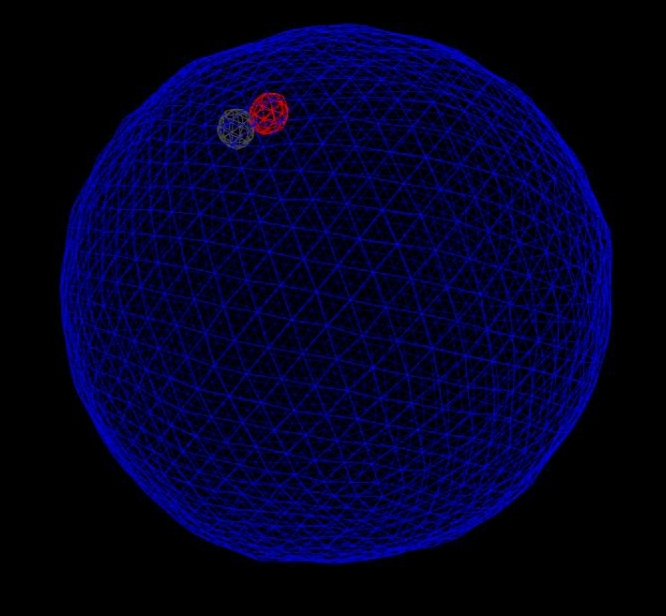
\includegraphics[width=9cm, height=9cm]{20210215_141728.jpg}
\end{center}\\




\section{\LARGE{جمع بندی}}
با توجه به نتایج شبیه سازی نشان داده شده دو نوع ساختار کلی غشا ی مایع و کشسان به وجود می آید. در برهمکنش غشا با ذرات غشا به عنوان یک واسطه موجب القای نیروی جاذبه میان نانوذرات میشود تا با صرف انرژی کمتر خمشی باعث کاهش انرژی کل سیستم شود.\\




\section{\LARGE{ارجاعات}}

%\bibitem{}
\lr{https://github.com/yeganeh1212/VCM-report/blob/main/config}\\
%20file.txt
%\bibitem{}
\lr{https://github.com/yeganeh1212/VCM-report/blob/main/FarsiThesis.pdf}\\
%\bibitem{}
\lr{https://github.com/yeganeh1212/VCM-report/blob/main/4_6046088568533682072.pdf}



%\end{thebibliography}









\end{document}